% $Header$

\documentclass{beamer}

% This file is a solution template for:

% - Talk at a conference/colloquium.
% - Talk length is about 20min.
% - Style is ornate.



% Copyright 2004 by Till Tantau <tantau@users.sourceforge.net>.
%
% In principle, this file can be redistributed and/or modified under
% the terms of the GNU Public License, version 2.
%
% However, this file is supposed to be a template to be modified
% for your own needs. For this reason, if you use this file as a
% template and not specifically distribute it as part of a another
% package/program, I grant the extra permission to freely copy and
% modify this file as you see fit and even to delete this copyright
% notice.


\mode<presentation>
{
  \usetheme{Warsaw}
  % or ...

  \setbeamercovered{transparent}
  % or whatever (possibly just delete it)
}


\usepackage[english]{babel}
% or whatever
\usepackage{tkz-euclide}
\usepackage[latin1]{inputenc}
% or whatever
\usepackage{xmpmulti}
\usepackage{times}
\usepackage[T1]{fontenc}
\usepackage{tikz}

% Or whatever. Note that the encoding and the font should match. If T1
% does not look nice, try deleting the line with the fontenc.
\addtobeamertemplate{navigation symbols}{}{%
    \usebeamerfont{footline}%
    \usebeamercolor[fg]{footline}%
    \hspace{1em}%
    \insertframenumber/\inserttotalframenumber
}
\setbeamercolor{footline}{fg=black}
\setbeamerfont{footline}{series=\bfseries}

\title[Sauce for the Goose is not Sauce for the Gander] % (optional, use only with long paper titles)
{Sauce for the Goose is not Sauce for the Gander}

\subtitle
{Assessing the Heterogeneous Impact of Climate Change on Bird Biodiversity in the United States}

\author[Luoye Chen] % (optional, use only with lots of authors)
{Luoye Chen\\ Madhu Khanna\inst{1}}
% - Give the names in the same order as the appear in the paper.
% - Use the \inst{?} command only if the authors have different
%   affiliation.

\institute[UIUC-ACE] % (optional, but mostly needed)
{
  \inst{1}%
  Department of Agricultural and Consumer Economics\\
  University of Illinois
}
% - Use the \inst command only if there are several affiliations.
% - Keep it simple, no one is interested in your street address.

\date[pERE 2018] % (optional, should be abbreviation of conference name)
{Grad Research Seminar, Nov 30th, 2018}
% - Either use conference name or its abbreviation.
% - Not really informative to the audience, more for people (including
%   yourself) who are reading the slides online

\subject{Environmental Economics}
% This is only inserted into the PDF information catalog. Can be left
% out.



% If you have a file called "university-logo-filename.xxx", where xxx
% is a graphic format that can be processed by latex or pdflatex,
% resp., then you can add a logo as follows:

% \pgfdeclareimage[height=0.5cm]{university-logo}{university-logo-filename}
% \logo{\pgfuseimage{university-logo}}



% Delete this, if you do not want the table of contents to pop up at
% the beginning of each subsection:
\AtBeginSubsection[]
{
  \begin{frame}<beamer>{OUTLINE}
    \tableofcontents[currentsection,currentsubsection]
  \end{frame}
}


% If you wish to uncover everything in a step-wise fashion, uncomment
% the following command:

%\beamerdefaultoverlayspecification{<+->}


\begin{document}

\begin{frame}
  \titlepage
\end{frame}

\begin{frame}{OUTLINE}
  \tableofcontents
  % You might wish to add the option [pausesections]
\end{frame}


% Structuring a talk is a difficult task and the following structure
% may not be suitable. Here are some rules that apply for this
% solution:

% - Exactly two or three sections (other than the summary).
% - At *most* three subsections per section.
% - Talk about 30s to 2min per frame. So there should be between about
%   15 and 30 frames, all told.

% - A conference audience is likely to know very little of what you
%   are going to talk about. So *simplify*!
% - In a 20min talk, getting the main ideas across is hard
%   enough. Leave out details, even if it means being less precise than
%   you think necessary.
% - If you omit details that are vital to the proof/implementation,
%   just say so once. Everybody will be happy with that.

\section{Motivation}

\subsection{Climate change and bird biodiversity}

\begin{frame}{WHY WORRY ABOUT BIRD BIODIVERSITY}{}
  % - A title should summarize the slide in an understandable fashion
  %   for anyone how does not follow everything on the slide itself.

  \begin{itemize}
  \item
    Biodiversity: measures of the joint dissimilarity among a set of species (Polasky,2005).
    \begin{itemize}
      \item Abundance: number of birds
      \item Species richness: number of bird species
      \item Species evenness: the level of how close in numbers each species in a community is
    \end{itemize}
  \item
   A source of economic and ecological opportunity
    \begin{itemize}
      \item Hunting and recreational value (Nocera and Koslowsky, 2017)
      \item Crucial ecosystem services (Frank,2018; Dissanayake and Ando, 2014)
      \item Indicators of the health of the environment (NABCI,2014)
    \end{itemize}

  \end{itemize}
\end{frame}

\begin{frame}
  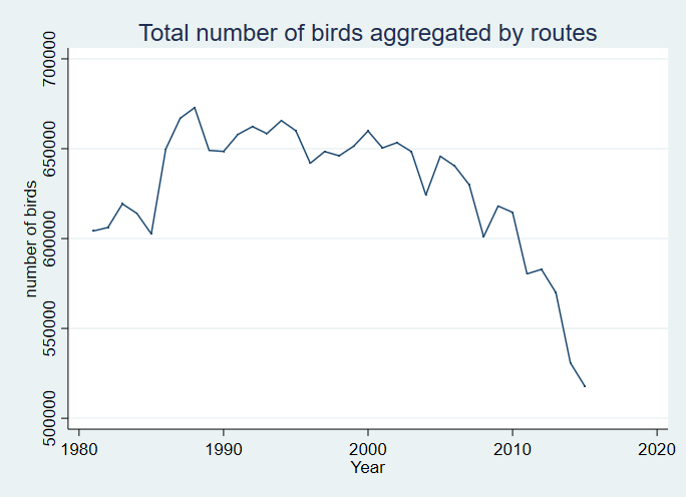
\includegraphics[width=0.8\textwidth]{bird-1.png}

  {\footnotesize  Source: North American Breeding Survey Data}
\end{frame}

\begin{frame}
  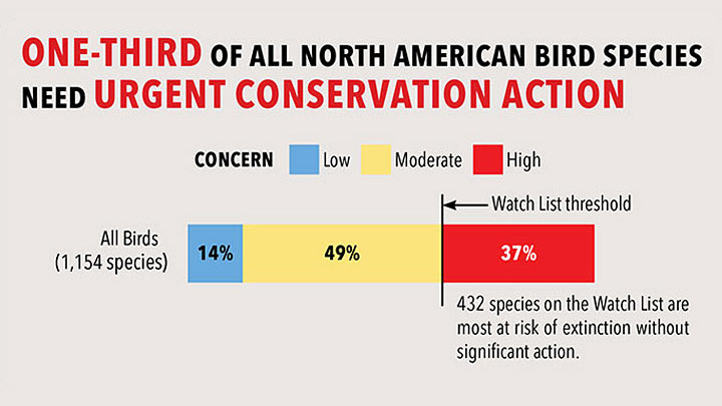
\includegraphics[width=0.8\textwidth]{bird-2.png}

  {\footnotesize  Source: North American Bird Conservation Initiative, U. S. Committee. 2016. The State of the Birds 2017: A Farm Bill Special Report. (http://www.stateofthebirds.org/2016/overview/results-summary/)}
\end{frame}


\begin{frame}{WHY WORRY ABOUT CLIMATE AND BIRD BIODIVERSITY}
  \begin{itemize}
    \item There are many reasons why climatic factors might influence birds
    \begin{itemize}
      \item Reduce reproductive and hatching success (Both and Visser, 2001; Miller-Rushing et al., 2008; Popoly et al., 2013)
      \item Advance the food peak (availability of insects) (McKechnie and Wolf, 2010; Welbergen e al., 2008)
    \end{itemize}
    \item Provide risk-management opportunities and quantify the net economic impact of changing climate condition on US's bird biodiversity.
    \item Relevant to the formation of US's national conservation policies.
  \end{itemize}
\end{frame}

\begin{frame}{RESERACH QUESTION}
  \begin{itemize}
    \item What is the quantitative evidence for a general linkage between climate and bird biodiversity
    \begin{itemize}
      \item Heterogeneity across bird metrics, species and regions
      \item Short-run and Long-run effect
    \end{itemize}
  \end{itemize}
\end{frame}

\subsection{Previous Work}

\begin{frame}{Identification Challenge I}
   \begin{itemize}
     \item Most of the climatic variables are exogenous (Dell et al., 2014)
     \item Cross-sectional variation (Hamer et al., 2006; Laaksonen and Lehikoinen, 2013; Illan et al., 2014)
   \end{itemize}
     \begin{block}{Unit Homogeneity Assumption (Burke and Emerick, 2016; Dell 2014; Hsiang, 2016)}
       Unobserved geographycal/geomorphology factors (e.g., elevation)
     \end{block}
\end{frame}

\begin{frame}{Identification Challenge II}
     \begin{itemize}
       \item Average temperature, precipitation (Review in Saether et al., 2004; Davey et al., 2012)
       \item Nonlinearity
     \end{itemize}
     \begin{block}{Marginal Treatment Comparability Assumption (Hsiang, 2016)}
     The effect of a marginal change in the distribution of weather is the same as the effect of an analogous marginal changes in the climate
     \end{block}
\end{frame}

\begin{frame}{Climate or weather?}
  \begin{figure}[h]
  %\caption{Table 1 Summary statistics}
  \centering
  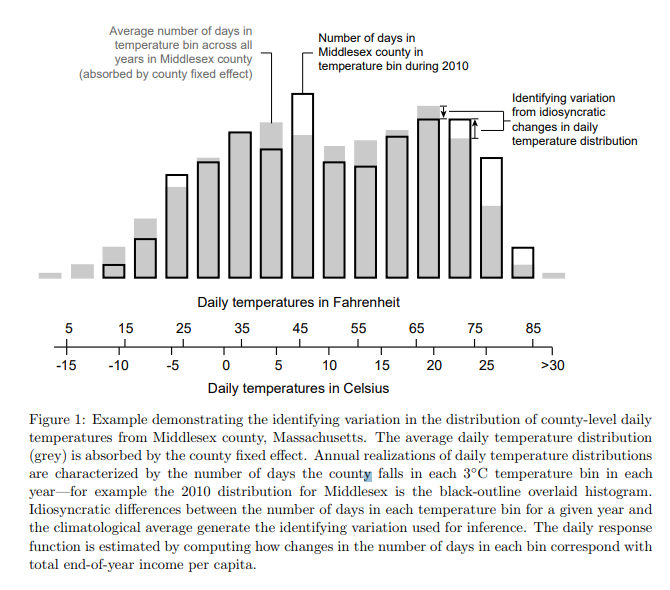
\includegraphics[width=0.6\textwidth]{climate_weather.png}
  \end{figure}
  Source: Deryugina \& Hsiang(2014)
\end{frame}


\begin{frame}{HYPOTHESIS}
  \begin{itemize}
    \item \alert{Hypothesis 1:}The abundance, species richness, and evenness of generalist birds will increase with additional high-tempearture days, while those of specialist birds will decrease with additional high-temperature days.
    \item \alert{Hypothesis 2:}Bird metrics (abundance, species richness, and species evenness) in the drier regions will respond more negatively to increase in the high-temperature days.
    \item \alert{Hypothesis 3:}The potential negative impact of an increase in the high-temperature days on bird abundance, species richness, and evenness will be mitigated in the long-run.
  \end{itemize}
\end{frame}


\section{Data and methods}
\begin{frame}{DATA}
  \begin{itemize}
    \item Northern American breeding bird survey (BBS) data
    \hyperlink{BBS routes}{\beamerbutton{here}}
    \begin{itemize}
      \item
      Annually survey data of bird population and species(1981-2015)
      \item
      3985 survey routes across the U.S.
      \item
      24.5-miles-long survey route with fifty stops situated ideally half-mile apart
      \item
      Time-varying convariates like sky or wind condition
    \end{itemize}
    \item NABCI species assessment database
    \item PRISM daily weather information $\rightarrow$ temperature bins
    \hyperlink{Temperature bins}{\beamerbutton{here}}
  \end{itemize}
\end{frame}

\begin{frame}{BBS route}
  \begin{figure}[h]
  %\caption{Table 1 Summary statistics}
  \centering
  \includegraphics[width=0.9\textwidth]{bbs_routes.png}
  \end{figure}
\end{frame}


\begin{frame}{Temperature bins}
  \begin{figure}[h]
  %\caption{Table 1 Summary statistics}
  \centering
  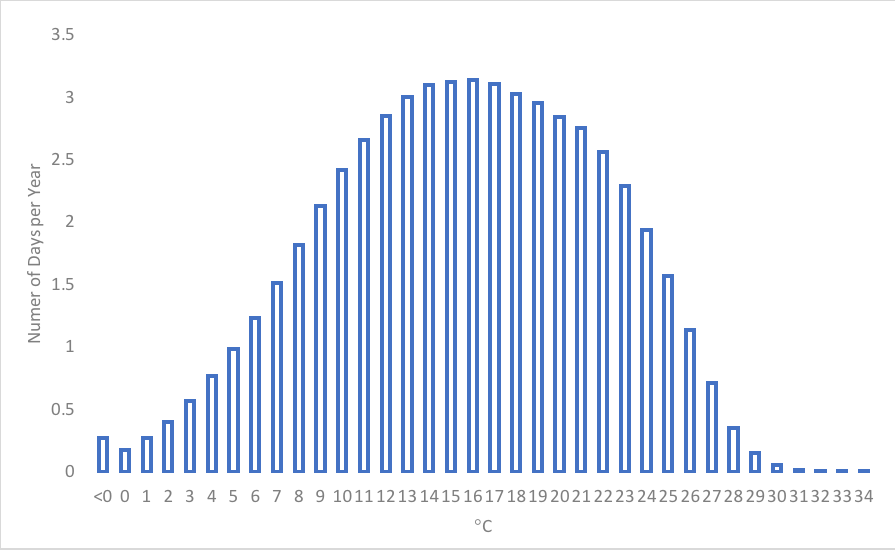
\includegraphics[width=0.9\textwidth]{temperature_bins.png}
  \end{figure}
\end{frame}

\begin{frame}{MODEL: Basic panel approach}
    \begin{equation}
      \begin{aligned}
        B_{i,t}=\alpha + \sum_{z=1}^{36} \textcolor{red}{\beta_{FE, z}} C_{i,t,z} + \gamma D_{i,t} + \mu_i + \phi_t + \epsilon_{i,t} \\ \textit{$i=1,...,N$ and $t=1,...,T$}
        \label{equ:e1}
      \end{aligned}
    \end{equation}
    \begin{block}{Identification Assumption}
    comparing the route i across 35 years; variation comes from the natural climate variability, especially the large differential warming trends observed over the United States. We assume the recent climate trends are exogenous.
   \end{block}
\end{frame}


\begin{frame}{Omitted variables concern: local land use}
    \begin{itemize}
      \item Bad control: Local land use change adjust to the climate
      \item No annual national-level land cover dataset
    \end{itemize}
    But we argue the omitted variable concerns would have a limited effect on identification based on:
    \begin{itemize}
      \item Lots of bird survey routes are located in the middle of forest and pasture lands; thereby expansion of residential housing land or cropland would have limited impact on them.
      \item Little change in either land area or land management practice (e.g., Burke and Emerick (2016a) use county-level data from 1950-2005)
      \item County-by-year fixed effect to absorb the shock from annual change of management practice in a specific county
    \end{itemize}
\end{frame}



\begin{frame}{MODEL: Long difference approach}
  \begin{itemize}
    \item Estimates of short-run responses to weather might not  bound estimates of longer run response to climate
\begin{equation}
    \Delta \bar{B}_{i,s} = \textcolor{red}{\beta_{LD}} \Delta \bar{C}_{i,s} + \textcolor{red}{\gamma_s} + \epsilon_{i,s}
    \label{equ:e2}
\end{equation}
In equation \eqref{equ:e2}, $\Delta \bar{B}_{i,s}$ is the change in bird metrics $B$ in route $i$ and region $s$ between two period $[t_a,t_b]$ far apart from each other.
\[
\Delta \bar{B}_{i,s} = \bar{B}_{i,t_b} - \bar{B}_{i,t_a} = \frac{1}{T} \sum_{t \in b} B_{i,t} - \frac{1}{T} \sum_{t \in a} B_{i,t}
\]
  \end{itemize}
\end{frame}

\begin{frame}{MODEL: Long difference approach}
    \begin{block}{Identification Assumptions}
      \begin{itemize}
        \item Comparing route i in region s across two periods far part in time (e.g., decades)
        \item Within-region variation, eliminating any concerns of time-trending unobservables at the region level (e.g., county level)
        \item We assume the climiate trends are exogenous.
      \end{itemize}
    \end{block}
\end{frame}


\begin{frame}{Long Difference}
%  \begin{tikzpicture}
%    \tkzInit[xmin=1983,xmax=2015]
%    \tkzGrid[sub,color=gray, subxstep=1]
%    \tkzAxeXY[very thick]
    %\tkzGrid
%  \end{tikzpicture}
\tikz{
 \node (a) at (0,0) {1981};
 \node (b) at (1.5,0) {1983};
 \node (c) at (3,0) {1985};
 \node (d) at (4.5,0) {...};
 \node (e) at (6,0) {2011};
 \node (f) at (7.5,0) {2013};
 \node (g) at (9,0) {2015};
 \node (h) at (1.5,-1) {$\frac{1}{5}\sum_{t=1981}^{1985}{Temp_i}$};
 \node (h) at (7.5,-1) {$\frac{1}{5}\sum_{t=2011}^{2015}{Temp_i}$};
 \node (i) at (4.5,-2) {$\Delta_{long \ diff}$};
 \draw[decoration={brace,mirror,raise=10pt},decorate]
  (0,0) -- (3,0) ;
 \draw[decoration={brace,mirror,raise=10pt},decorate]
   (6,0) -- (9,0) ;
  \draw[decoration={brace,mirror,raise=10pt},decorate]
     (1.5,-1) -- (7.5,-1) ;
}
\end{frame}

\section{Results}

\subsection{Main Results}

\begin{frame}{Main Result}
  \begin{figure}[h]
  %\caption{Table 1 Summary statistics}
  \centering
  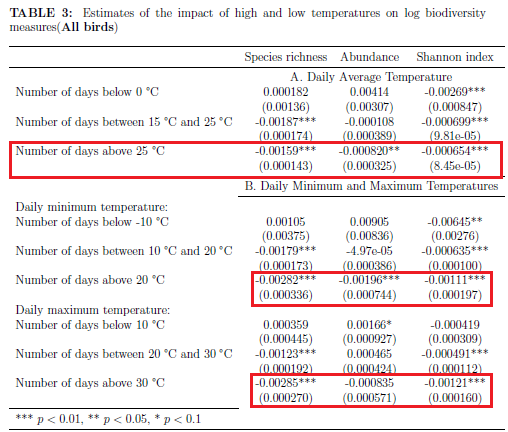
\includegraphics[width=0.7\textwidth]{main_result.png}
  \end{figure}
\end{frame}

\begin{frame}{Statistical testing: does $\beta_{FE}$ close to $\beta_{LD}$}
  \begin{itemize}
    \item \%Adaptation = $1-\frac{\beta_{LD}}{\beta_{FE}}$
  \end{itemize}
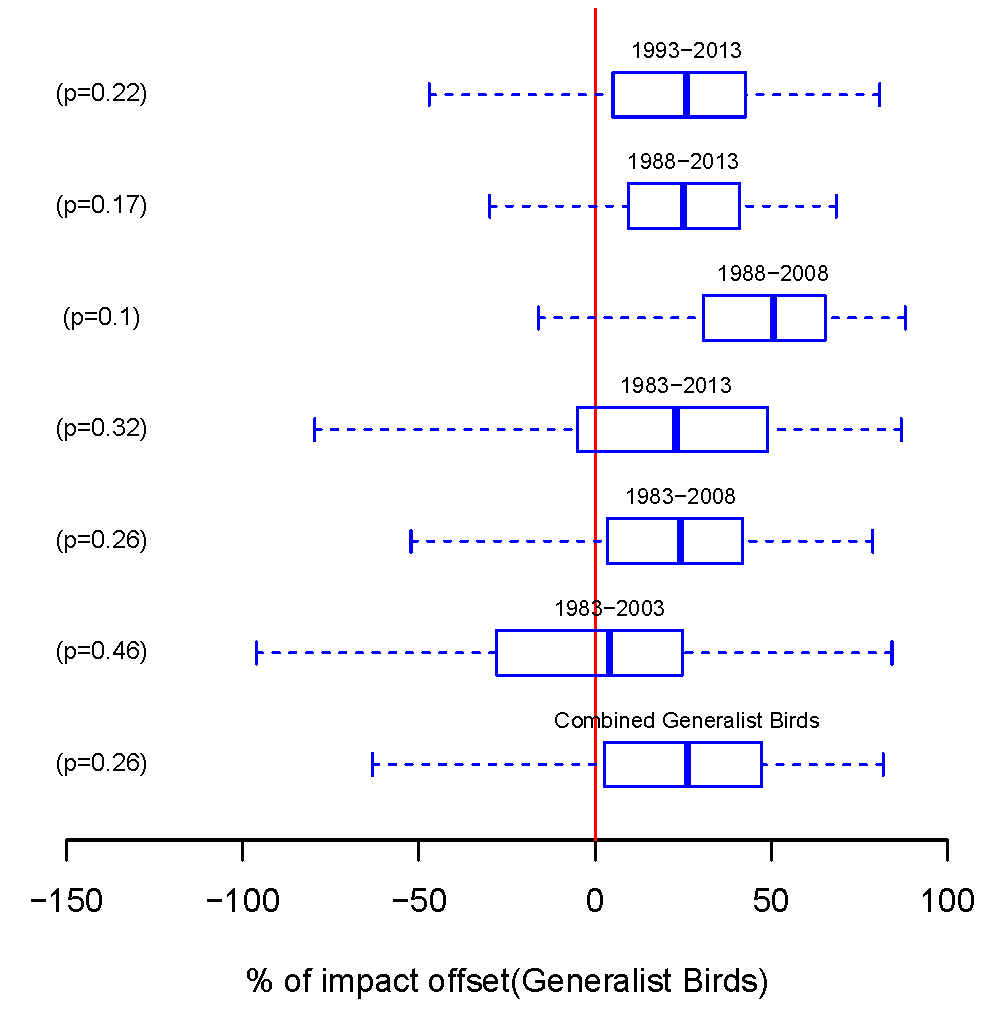
\includegraphics[width=0.5\textwidth]{long_diff1.png}%
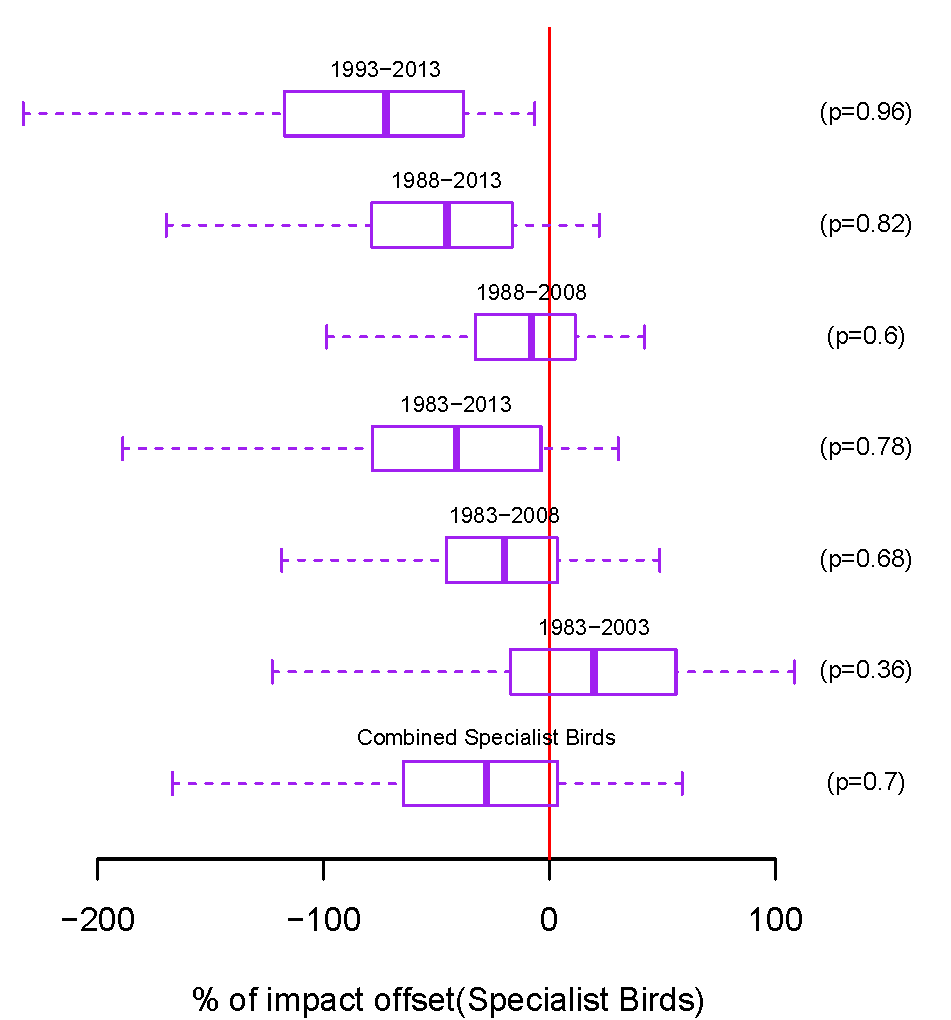
\includegraphics[width=0.5\textwidth]{long_diff2.png}
\end{frame}

\begin{frame}{Mechanism: Different Measures-Decomposition}
  \begin{figure}[h]
  %\caption{Table 1 Summary statistics}
  \centering
  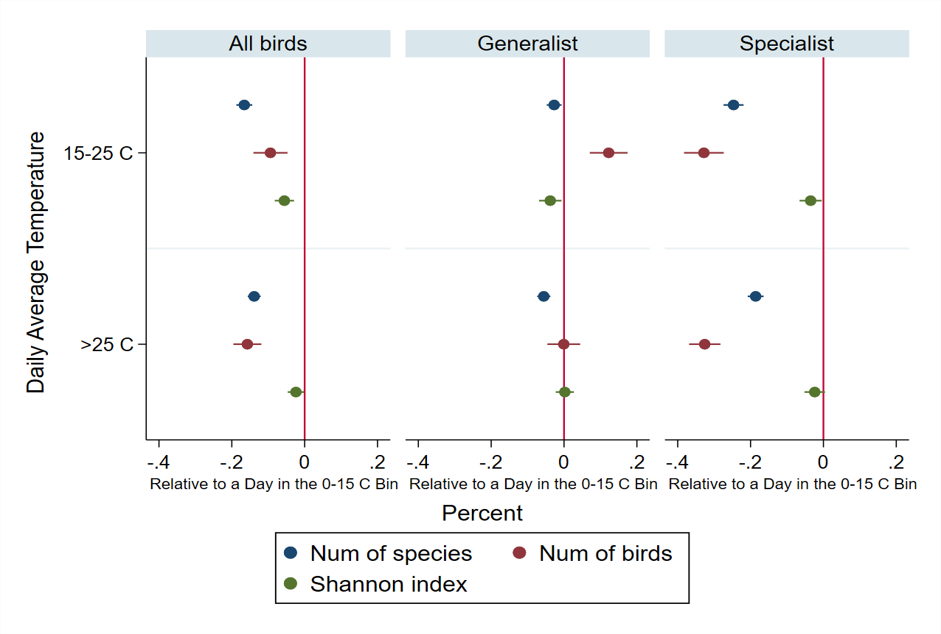
\includegraphics[width=0.9\textwidth]{result_mreasure1.png}
  \end{figure}
\end{frame}

\begin{frame}{Mechanism: Different Measures-Decomposition(con't)}
%  \begin{figure}[h]
  %\caption{Table 1 Summary statistics}
%  \centering
  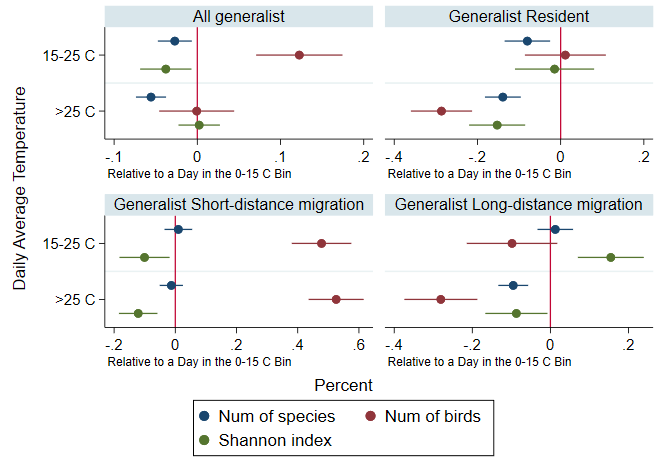
\includegraphics[width=0.5\textwidth]{bird_figure2b}%
  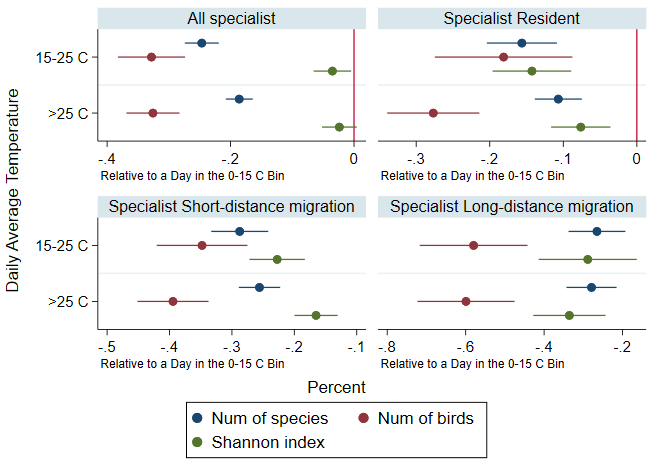
\includegraphics[width=0.5\textwidth]{bird_figure2c}
%  \end{figure}
\end{frame}

\begin{frame}{Mechanism: Different species/regions}
  \begin{figure}[h]
  %\caption{Table 1 Summary statistics}
  \centering
  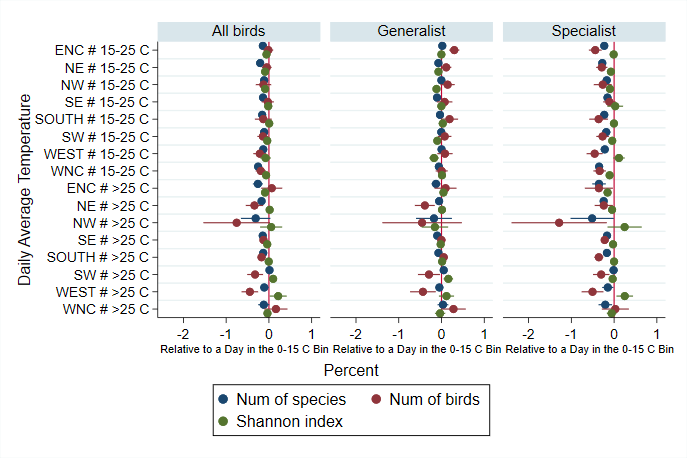
\includegraphics[width=0.9\textwidth]{bird_figure3.png}
  \end{figure}
\end{frame}

\begin{frame}{Robustness Check}
 \begin{itemize}
   \item Daily tempearture exposure windows: 2/3/6 months
   \item Choice of time periods: 5/10/15/20/25 spanning years
   \item Temperature bins: 1/5/10 �C bins
   \item Measurement error
   \item Distributed Lag model
   \item Clustering: robust/county + year-by-state/ecoregion
   \item Outliers
 \end{itemize}
\end{frame}



\section*{SUMMARY}

\begin{frame}{Summary}

  % Keep the summary *very short*.
  \footnotesize
  \begin{itemize}
  \item
  Overall, for the whole bird group, increase in the high-temperatuer days had a significant impact on biodiversity of bird species in routes that were distributed across the United States.
  \item The long-run adaptation has offset only 20\% of the negative short-term impact of extreme heat(>25 �C) on bird species richness. Birds has no more adaptation to extreme heat in the long run.
  \item
    Swapping a standard deviation of days in the 0-15 �C range for ones above 25 �C increases the decline of bird abundance, species richness and evenness by approximately 1\%~2.5\%.
  \item
  The impact of additional extreme heat temperature days (>25 �C degree) on specialist birds is almost three times larger than the generalist birds.
  \item
  Effect in the western and northern region will be more negative on the bird abundance(-1.5\%), species richness(-0.6\%) and Shannon-weaver index(-0.6\%).
  \end{itemize}
\end{frame}

\begin{frame}{Summary}
  \item The average WTP to pay for each bird species in one birding trip is \$3.38 [1.97, 4.88] (Kolstoe and Cameron, 2017).
  \item In 2011, the Oregon state and Washing States has 4 million and 5.2 million birding trips, respectively (FHWAR survey, 2011).
  \item The economic loss yields average \$18 million.
\end{frame}

\end{document}
